\documentclass[12pt]{report}
% Definiciones basicas de LaTeX para la memoria
%
% No modificar las lineas a continuacion a menos
% de estar muy seguro de lo que se esta haciendo!!
%
% Jaime Cisternas, julio 2004, agosto 2010

% <jcisternas@uandes.cl> 

%%%%%%%%%%%%%%%%%%%%%%%%%%%%%%%%%%%%%%%%%%%%%%%%%%%%%%%%%%%%%%%%%%%%%
% Libreria computin
%\usepackage{algorithm}
%\usepackage{algorithmic}
\usepackage[left=3cm,top=2.5cm,right=3cm,bottom=2.5cm]{geometry}

% Encoding

\usepackage[utf8]{inputenc}

% Carga librerias utiles con simbolos y estructuras
\usepackage{amsfonts}
\usepackage{amssymb}
\usepackage{amsmath}   
\usepackage{amsthm}
\usepackage{latexsym}
\usepackage{cancel}
\usepackage{physics}
\usepackage{bbm}

% Librerías adicionales para diagramas tikz

\usepackage{tikz}
\usepackage{mathdots}
\usepackage{yhmath}
\usepackage{color}
\usepackage{siunitx}
\usepackage{multirow}
\usepackage{gensymb}
\usepackage{tabularx}
\usepackage{extarrows}
\usepackage{booktabs}
\usetikzlibrary{fadings}
\usetikzlibrary{patterns}
\usetikzlibrary{shadows.blur}
\usetikzlibrary{shapes}


% Libreria para ajustar espaciado entre lineas
\usepackage{setspace}

% Libreria con estilo APA para bibliografia
\usepackage{core/newapa}

% Si usted está utilizando un teclado en español, puede ser útil
% usar los paquetes a continuacion. De otra manera tendrá que generar las
% tildes y la letra ñ de forma especial.
% Estos caracteres no pueden ser utilizados en etiquetas ni tampoco en modo matemático
\usepackage[spanish, activeacute]{babel}
\unaccentedoperators


% Declaraciones especificas de pdfLaTeX
\usepackage[pdftex,
        colorlinks=false,         % true or false (for final version)
        urlcolor=rltblue,         % \href{...}{...} external (URL)
	    anchorcolor=rltbrightblue,
        filecolor=weben,          % \href*{...} local file
        linkcolor=webred,         % \ref{...} and \pageref{...}
        menucolor=webdarkblue,
        citecolor=webgreen,
        pdftitle={},              % INSERT YOUR TITLE HERE
        pdfauthor={},             % INSERT YOUR NAME HERE
        pdfsubject={},
        pdfkeywords={},
        pdfpagemode=None,
        bookmarksopen=true,
	plainpages=false]{hyperref}
%\usepackage[pdftex]{graphicx}

\usepackage{graphicx}


\pdfcompresslevel=9
\pdfadjustspacing=1
% Definicion de colores
\usepackage{color}
\definecolor{rltbrightred}{rgb}{1,0,0}
\definecolor{rltred}{rgb}{0.75,0,0}
\definecolor{rltdarkred}{rgb}{0.5,0,0}
\definecolor{rltbrightgreen}{rgb}{0,0.75,0}
\definecolor{rltgreen}{rgb}{0,0.5,0}
\definecolor{rltdarkgreen}{rgb}{0,0,0.25}
\definecolor{rltbrightblue}{rgb}{0,0,1}
\definecolor{rltblue}{rgb}{0,0,0.75}
\definecolor{rltdarkblue}{rgb}{0,0,0.5}
\definecolor{webred}{rgb}{0.5,.25,0}
\definecolor{webblue}{rgb}{0,0,0.75}
\definecolor{webgreen}{rgb}{0,0.5,0}
\definecolor{webdarkblue}{rgb}{0,0,0.5}
\definecolor{webbrightgreen}{rgb}{0,0.75,0}
% fin de declaraciones especificas pdfLaTeX

% tamanio de pagina
%\setlength{\oddsidemargin}{.5in}
%\setlength{\evensidemargin}{.0in} % en caso de usar opcion 'twoside'
%\setlength{\textwidth}{6in}
%\setlength{\topmargin}{-.5in}
%\setlength{\textheight}{9in}


% Las siguientes definiciones pueden ser usadas en
% memorias mas matematicas
\newtheorem{theorem}{Teorema}[section]
\newtheorem{lemma}[theorem]{Lema}
\newtheorem{corollary}[theorem]{Corolario}
\newtheorem{proposition}[theorem]{Proposición}
\newtheorem{definition}[theorem]{Definición}
\newtheorem{claim}{Afirmación}
\newtheorem{conjecture}[theorem]{Conjetura}
\newtheorem{observation}[theorem]{Observación}
\newtheorem{problem}[theorem]{Problema}

% Definicion de un ambiente para algoritmos en pseudo-codigo.
% Esta definicion puede ser mejorada.
\newtheorem{algorithm}{Algoritmo}[section]
\newcommand{\tab}{\hspace*{0.5 cm}}
% Palablas claves que deben aparecer en negrita
\newcommand{\bfWHILE}{\textbf{while~}}
\newcommand{\bfDO}{\textbf{do~}}
\newcommand{\bfEND}{\textbf{end~}}
\newcommand{\bfIF}{\textbf{if~}}
\newcommand{\bfTHEN}{\textbf{then~}}
\newcommand{\bfELSE}{\textbf{else~}}
\newcommand{\bfFOR}{\textbf{for~}}

% Nombres fijos de Latex pueden ser cambiados al Espaniol
\renewcommand{\contentsname}{Índice General}
\renewcommand{\chaptername}{Capítulo}
\renewcommand{\appendixname}{Anexo}
\renewcommand{\bibname}{Bibliografía}
\renewcommand{\figurename}{Ilustración}
\renewcommand{\tablename}{Tabla}
\renewcommand{\indexname}{Índice}
\renewcommand{\partname}{Parte}
\renewcommand{\listfigurename}{Lista de Ilustraciones}
\renewcommand{\listtablename}{Lista de Tablas}

% Para las enumeraciones usamos primero a,b,c,... y despues i, ii, iii,...
\renewcommand{\labelenumi}{\alph{enumi})}
\renewcommand{\labelenumii}{\roman{enumii})}
\renewcommand{\labelenumiii}{-}
\renewcommand{\labelenumiv}{-}

% Para ser consistentes en el uso de abreviaciones!
%\newcommand{\Chp}{Cap\'{\i}tulo}
%\newcommand{\Chps}{Cap\'{\i}tulos}
%\newcommand{\Sec}{Sec.} % \S
%\newcommand{\Secs}{Secs.} % \S\S
%\newcommand{\SSec}{Subsec.}
%\newcommand{\Fig}{Fig.}
%\newcommand{\Figs}{Figs.}
%\newcommand{\Eqn}{Ecn.}
%\newcommand{\Eqns}{Ecns.}

% Muestra en pantalla los nombres de los archivos usados
\listfiles

% Previene una cierta senial de ``warning: contentsline with no destination''
\newcounter{dummy}



\setlength{\parindent}{0cm}
\usepackage{float}
\usepackage{subfigure}
\usepackage{array}
\newcolumntype{E}{>{$}c<{$}}
\usepackage{longtable}
\setcounter{MaxMatrixCols}{40}
\usepackage{bm}

%%%%%%%%%%%%%%%%%%%%%%%%%%%%%%%%%%%%%%%%%%%%%%%%%%%%%%%%%%
\newcommand{\nombreautor}{Alumnos}
\newcommand{\mes}{Mes}
\newcommand{\anio}{Año}
\newcommand{\titulo}{Título}
\newcommand{\nombreprofuno}{Sebastián Cea Echenique}
\newcommand{\nombreprofdos}{Nombre Profe 2}
\newcommand{\nombreproftres}{Nombre Profesor Invitado}
\newcommand{\codigo}{ING-IN-001/11}

%%%%%%%%%%Aqui se escribe el resumen%%%%%%%%%%%%%%%%%%%%%
\newcommand{\resumen}{
Hacer resumen al terminar la tesis. Máximo 1 página
}

\newcommand{\agradecimientos}{
Muchas gracias a todos}

\newcommand{\dedicatoria}{\it
ok..
}
\renewcommand{\baselinestretch}{1.5}

%%%%%%%%%%%%%%%%%%%%%%%%%%%%%%%%%%%%%%%%%%%%%%%%%%%%%%%%%%

% Por favor coloque todas las definiciones de simbolos a continuacion
% y no en los archivos de capitulos. Esto evitara la  existencia de
% multiples definiciones para las mismas palabras.

\newcommand{\mydef}
	{\stackrel{\mathrm{def}}{=}}
\newcommand{\e}
	{\hbox{\large{e}}}
\newcommand{\mi}
	{\hbox{\large{i}}}
\newcommand{\RR}{\mathbb{R}}


%%%%%%%%%%%%%%%%%%%%%%%%%%%%%%%%%%%%%%%%%%%%%%%%%%%%%%%%%%

\begin{document}
\label{start}

% Genera las paginas de titulo, copyright, resumen,
% agradecimientos, dedicatoria, indices,...

% No es necesario modificar

% Paginas de titulo, derechos de autor y otras mas.

% Jaime Cisternas, julio 2004, agosto 2010

% declaracion especifica de pdfLaTeX
% permite incluir figuras con \includegraphics[...]{figurename}
\DeclareGraphicsExtensions{.jpg,.pdf,.mps,.png}

%%%%%%%%%%%%%%%%%%%%%%%%%%%%%%%%%%%%%%%%%%%%%%%%%%%%%%%%%%%%%%%%

  \pagenumbering{roman}
% \setcounter{page}{1}

% Escribe la pagina de titulo, incluyendo el autor y la facultad

  \thispagestyle{empty}
  \textsc{
  \vspace*{0cm}
  \begin{center}
    \Large
     Universidad de los Andes \\
     Facultad de Ingeniería y Ciencias Aplicadas\\
  \end{center}
     \vspace{1cm}
  \begin{center}
     
\includegraphics[angle=0,height=5cm]{logos/Logo-UANDES.png}
  \end{center}
     \vspace{1cm}
  \begin{center}
     \Large
     \titulo
  \end{center}
  \vspace{0.5cm}
  \begin{center}
    \Large
    \nombreautor
  \end{center}
  \vspace{0.5 cm}
  \begin{center}
    Memoria para optar al título de \\
    Ingeniero Civil Industrial 
    Mención Ingeniería Financiera\\
    \vspace{1cm}
    Profesor Guía: \nombreprofuno \\
    Profesor Co-Guía: \nombreprofdos \\
    \vspace{0.5cm}
    \codigo \\
    \vspace{0.5cm}
    Santiago, \mes\ de \anio
  \end{center}
  }

%%%%%%%%%%%%%%%%%%%%%%%%%%%%%%%%%%%%%%%%%%

% Escribe la segunda pagina de titulo para ser firmada por la comision

\cleardoublepage
\thispagestyle{empty}

\begin{center}

\vspace*{2cm}
\parbox{10cm}{
\noindent
Certifico que he leído esta tesis y que en mi opinión
su alcance y calidad son completamente adecuados como para ser considerada
una tesis conducente al título de Ingeniero y grado de Magíster.
\vspace{1cm}

\hfill
\begin{tabular}{c}
\hspace{8cm} \\
\hline
\nombreprofuno \\
(Profesor Guía)
\end{tabular}

\vspace*{1.5cm}

\noindent
Certifico que he leído esta tesis y que en mi opinión
su alcance y calidad son completamente adecuados como para ser considerada
una tesis conducente al título de Ingeniero y grado de Magíster.
\vspace{0.75cm}

\hfill
\begin{tabular}{c}
\hspace{8cm} \\
\hline
\nombreprofdos
\end{tabular}

\vspace*{1.5cm}

\noindent
Certifico que he leído esta tesis y que en mi opinión
su alcance y calidad son completamente adecuados como para ser considerada
una tesis conducente al título de Ingeniero y grado de Magíster.
\vspace{0.75cm}

\hfill
\begin{tabular}{c}
\hspace{8cm} \\
\hline
\nombreproftres
\end{tabular}
}

\end{center}

%%%%%%%%%%%%%%%%%%%%%%%%%%%%%%%%%%%%%%%%%%

% Espaciado entre lineas
  \onehalfspacing
  %\doublespacing

% Hace pagina de derechos de autor

  \cleardoublepage
  \thispagestyle{empty}
  %\vspace*{0in}
  \begin{center}
    \copyright\ \nombreautor\ \anio \\
    Todos los derechos reservados.
  \end{center}

%%%%%%%%%%%%%%%%%%%%%%%%%%%%%%%%%%%%%%%%%%%%%%%%%%%%%%%%%%%%%%%%%%%%%%

% Genera resumen leyendo definicion de resumen

  \cleardoublepage
  \refstepcounter{dummy} \addcontentsline{toc}{section}{Resumen}
  \begin{center} \Large \textbf{Resumen} \end{center}
  \resumen

% Genera agradecimientos leyendo definicion de agradecimientos

  \cleardoublepage \addcontentsline{toc}{section}{Agradecimientos}
  \begin{center} \Large \textbf{Agradecimientos} \end{center}
  \agradecimientos

% Genera dedicatoria

  \cleardoublepage \vspace*{1.5in}
  \begin{flushright} \dedicatoria \end{flushright}

% Produce indice general, listas de figuras y de tablas

  \cleardoublepage
  \tableofcontents
  \cleardoublepage
  \listoffigures
  \cleardoublepage
  \listoftables
  \cleardoublepage

  \normalsize
  \pagenumbering{arabic}

%%%%%%%%%%%%%%%%%%%%%%%%%%%%%%%%%%%%%%%%%%%%%%%%%%%%%%%%%%%


%%%%%%%%%%%%%%%%Ingreso de capitulos%%%%%%%%%%%%%%%%%%%%%%

% cap1.tex

\chapter{Introducción}
\label{c1} % la etiqueta para referencias

En la actualidad, se reconoce a nivel mundial que el planeta está experimentando un cambio climático potencialmente perjudicial para la vida en él. También, múltiples estudios científicos y gran parte de la sociedad concuerdan en que muchas de las actividades del ser humano son un acelerador significativo de este cambio y el aumento de la temperatura. De acuerdo con diversos estudios, esto último apunta a que el aumento global de temperatura se debe al efecto invernadero, principalmente producido por $CO_2$. Este es un componente generado en un gran volumen por las actividades humanas tales como el transporte, la generación de energía, la ganadería, entre otros.
\vspace{2.5mm}

Esta situación ha generado un incentivo en las personas para encontrar soluciones y reducir el factor humano en el cambio climático. Con esto, se han producido importantes innovaciones y cambios en las industrias mencionadas y también se ha impulsado la creación de sistemas que permitan que estas transiciones sean sustentables y realistas en el largo plazo. 
\vspace{2.5mm}

Específicamente en Chile, la Estrategia climática de largo plazo de Chile (ECLP) presentada en el año 2021 por el Ministerio del Medio Ambiente concluye que el sector energético representó un 77\% de los gases de efecto invernadero producidos  en el año 2018 y, en ese sector, la generación de energía representa el mayor aporte con un 30\% del total de emisiones. Con el fin de disminuir este porcentaje, existen alternativas de generación más limpia que en la actualidad se emplean mayoritariamente. Sin embargo su implementación y producción es aún, en la mayoría de los casos, menos rentable, aunque la trayectoria de estas tecnologías muestra que, potencialmente, esto cambiará de forma positiva.
\vspace{2.5mm}

No obstante el trabajo realizado por \citeB{amigo_two_2021} demuestra que, con el sistema actual de penalización de emisiones que regula la industria generadora de electricidad, no es suficiente para lograr un cambio significativo y la reducción necesaria para lograr las metas prepuestas por Chile en el Acuerdo de París ni en el ECLP. Por lo tanto, los autores proponen un sistema de \emph{cap and trade} de dos etapas con mercado de compra y venta de permisos de contaminación. En este, las metas sí se logran cumplir y demuestra cómo es el efecto de este sistema con distintos presupuestos de contaminación. Sin embargo, este modelo propuesto presenta algunas limitaciones y posibilidades de mejora, que este trabajo busca aportar, específicamente sobre el problema del \emph{auctioneer} (subastador en inglés) de estos permisos de contaminación.


\section{Motivación}
Encontrar un modelo óptimo y eficiente para implementar en la industria de energía parece ser una tarea difícil. Muchos países tienen la intención de rebajar su aporte de contaminante global para alcanzar el acuerdo de París, pero una iniciativa no es suficiente, si no se respalda con continuo cambio y mejora. Cualquier tipo de modelo implementado a gran escala, como la fiscalización de la industria eléctrica, requiere de evaluación continua y estudio de implementaciones en otros países para encontrar cuál es la mejor solución al problema.
\vspace{2.5mm}

El ECLP dicta que Chile tiene como objetivo ser carbono neutral\footnote{Carbono neutral no significan 0 toneladas de dióxido de carbono emitidas, sino que las emisiones sean iguales a las absorciones por agentes como el sector forestal.} como fecha límite para el año 2050. A la fecha, el país tiene como estrategia para disminuir las emisiones de la industria eléctrica aplicar un ``impuesto verde'' descrito en la ley 20.780 promulgada en el año 2014. Diversos estudios (mencionados en el marco teórico de este trabajo) argumentan que esto no es suficiente y su aplicabilidad no es sustentable y no incentiva el cambio a energías renovables. En efecto, los autores \citeB{amigo_two_2021} demuestran y concluyen que, en primer lugar, el objetivo de carbono neutralidad es lograble y, en segundo lugar, que el \emph{National Determined Contribution}  (NDC por sus siglas en inglés)\footnote{National Determined Contribution: Aporte del país en la propuesta del acuerdo de París}  propuesto para el acuerdo de París\footnote{En el acuerdo de París se estableció como objetivo no superar un aumento global de temperatura de 2 °C para finales de este siglo.}, que consiste en que, para el año 2030, el nivel de $CO_2 e$ (dióxido de carbono emitido) no supere los 131 $MtCO_2 e$ en Chile, es una meta fácil de lograr y, por lo tanto, ineficiente. Ellos proponen la implementación de una versión de su modelo de \emph{cap and trade}, con la cuál se pueden alcanzar objetivos mucho más ambiciosos en la reducción de emisiones y sobre el cambio a una generación de energía con fuentes sustentables.
\vspace{2.5mm}

Entonces, el propósito de este trabajo es aportar en la investigación, testeo y extensión del modelo por medio de la incorporación del concepto de inatención (o atención) racional. Como hipótesis se tiene que la falta de atención impacta negativamente en el cumplimiento de las métricas de reducción de amisiones de carbono.
\vspace{2.5mm}

En adición a lo anterior, se busca entender el efecto de su implementación en el modelo y concluir si este presenta potencialidad para disminuir las emisiones de carbono y así aumentar el bienestar social.


\section{Objetivos}
\subsection{Objetivo general}
El objetivo general de este trabajo es reformular el modelo de \textit{cap and trade} de dos etapas creado por \citeB{amigo_two_2021} por medio de la incorporación del concepto de atención racional  y evaluar su efecto en las emisiones de carbono en la industria eléctrica . 

\subsection{Objetivos específicos}
Los objetivos específicos necesarios para lograr el objetivo general son:

\begin{enumerate}
\item Identificar modelos de equilibrio y modelos de equilibrio en capacidad.
\item Identificar métodos de resolución de \emph{Mixed Complementarity Problems} (MCP).
\item Programar problemas MCP en GAMS.
\item Replicar el modelo original de \citeB{amigo_two_2021}.
\item Implementar atención racional en el modelo.
\item Resolver el nuevo modelo y analizar resultados.
\end{enumerate}


\section{Alcances}

Los alcances de este trabajo son: estudiar con profundidad los modelos de equilibrio en capacidad. Resolver problemas complejos de tipo MCP como mínimo en un lenguaje de programación y un \textit{solver}. Replicar el modelo de \textit{cap and trade} propuesto por \citeB{amigo_two_2021}. Como alcance final, se tiene, implementar el concepto de atención racional en el modelo como mínimo en una reformulación del modelo y proporcionar su resolución y compración con el modelo original. 
\vspace{2.5mm}

Debido a que este este es un concepto novedoso, queda fuera del alcance de este trabajo la proporción de un modelo con atención racional de implementación real en Chile. Se espera obtener resultados suficientes para incentivar su mejora y posterior versión con implicaciones reales.

\section{Metodología}
Con el fin de cumplir los objetivos y alcances de este trabajo se lleva a cabo la siguiente metodología:

\begin{enumerate}
\item Identificar modelos de equilibrio y modelos de equilibrio en capacidad. Como base se tomó la bibliografía recomendada por el profesor guía junto con filtros según estándares académicos de impacto y otras características. De esta forma, se lleva a cabo un estudio de los modelos de equilibrio.

\item Identificar métodos de resolución de MCP: para resolver los problemas de equilibrio es posible transformarlos en MCP al aplicar las condiciones de Karush-Kuhn-Tucker (KKT). Se estudió principalmente de un curso realizado por Felipe Feijoo en el verano del año 2022 llamado ``Computo de modelos de equilibrio", organizado por Sebastián Cea y la facultad de ingeniería de la Universidad de los Andes.\footnote{Material audiovisual disponible en \url{https://youtube.com/playlist?list=PLeAzsOHIpDozzT59xbM-MGIU8_uwLZsAA}}   

\item Programar problemas MCP: es necesario aprender sobre distintos solvers de MCP y softwares que lo soporten. Primero, se realizan ensayos de programación con problemas de similar naturaleza al de \citeB{amigo_two_2021} en \citeB{d__aertrycke_risk_2017}. Finalmente, se busca profundizar con el curso de Felipe Feijoo sobre MCP. 

\item Replicar modelo original de Amigo: se desarrollan las condiciones de KKT y formulación de MCP para resolver el modelo original. Luego, se ejecuta el código original con los parámetros utilizados en el \textit{paper} para visualizar resultados y entender el funcionamiento.

\item Implementar el concepto de atención racional al modelo: se reformula el modelo incoporando el concepto de atención racional.

\item Evaluar nuevo modelo en \textit{solver} y analizar resultados: se evalúa el nuevo modelo al ejecutarlo en un \textit{solver} y se analizan las variables óptimas encontradas.
\end{enumerate}

\newpage
\section{Estructura del documento}

La estructura del documento se divide en cinco capítulos: introducción, marco teórico, desarrollo metodológico, análisis de resultados y conclusiones.
\vspace{2.5mm}

El presente capítulo introductorio que tiene como objetivo contextualizar al lector sobre la estructura general e implicancias de este trabajo.
\vspace{2.5mm}

El marco teórico presenta el estudio realizado anterior a la implementación del concepto de atención racional en el modelo. En este se definen los problemas de equilibrio, MCP y la condiciones de KKT. Se presenta un tutorial para resolver problemas no lineales en distintos lenguajes de programación y \textit{solvers}. También se explica el trabajo realizado por \citeB{amigo_two_2021} y el concepto de atención racional.
\vspace{2.5mm}

En el desarrollo metodológico se replica el modelo original y luego se reformula en dos versiones nuevas. En adición a esto, se realiza la traducción del problema original al lenguaje de programación \julia con el fin de agilizar futuras resoluciones. En particular, \julia resulta ser más eficiente\footnote{Sólo menos ineficiente que C, ver \url{https://julialang.org/benchmarks/}} en el cómputo y en la automatización del análisis de resultados.
\vspace{2.5mm}

El capítulo 4 muestra los resultados de la replicación del modelo original y de los nuevos modelos formulados en el capítulo anterior. Se proporciona un análisis de estos y su comparación con el modelo original.
\vspace{2.5mm}

Finalmente, en el capítulo 5, se concluye si las nuevas versiones del modelo, que incorporan el concepto de atención racional, presenta resultados suficientes para su posterior mejora y presentación de un modelo de implementación real en Chile.




% cap2.tex

\chapter{MARCO TEÓRICO}\label{Marco Teorico}
\section{\textit{Amigo et alii} y \textit{papers} relacionados}

REVISAR REVICION BIBLIOGRÁFICA HITO 1, OJO QUE HAY PARRAFOS USADOS PARA EL CAPITULO 1 DE ESTE LIBRO.


\label{c2} % la etiqueta para referencias




TEXTO

%% cap3.tex

\chapter{Desarrollo Metodológico} \label{MCP:subastador} % la etiqueta para referencias


\section{Replicación del modelo original y resolución por medio de MCP}

Una de las formas de resolver el problema original de \citeB{amigo_two_2021}, debido a que este es un problema de equilibrio con varios modelos involucrados, es transformar cada modelo en MCP y resolverlos juntos. Gracias a las variables duales, estos modelos se relacionan. La transformación a MCP es posible gracias al teorema de Karush-Kuhn-Tucker, explicado en el Capítulo \ref{descripcionkkt}, y sus condiciones resultantes. 
\vspace{2.5mm}

Por lo tanto, para replicar el modelo original, se realiza esta transformación para el problema del subastador (el MCP de los productores se desarrolló en el Capítulo \ref{MCPproductor} y el MCP condiciones de mercado en el Capítulo \ref{MCPmercado}). Finalmente, esta es traducida en un \textit{solver} para evaluar y comparar sus resultados con el original.

\subsection{MCP problema del subastador} \label{MCPsubastador}

Además de lo realizado con el problema del productor y las restricciones de las condiciones de mercado, que relacionan a los productores con el subastador, se debe transformar el problema de este último (mostrado en el modelo \ref{eq:sub}) en un MCP.  Para comenzar, se obtiene el lagrangeano del problema:

\begin{footnotesize}
\begin{align}
\mathcal{L}(\theta) = -\theta\pi^a + \mathcal{F}(\theta) - \eta (\varphi^-1(M)\sigma+\mu-\theta) - \varrho(\theta)  \label{eq:lagrange2}
\end{align}
\end{footnotesize}


\subsubsection{Derivada parcial respecto a $\theta$}

Debido a que $\theta$ es la única variable del modelo, se debe realizar solamente la derivada del lagrangeano respecto a esta. Se obtiene lo siguiente:

\begin{footnotesize}
\begin{align}
    \frac{\partial \mathcal{L}(\theta) }{\partial \theta} = 0 =  -\pi^a + \frac{\partial\mathcal{F}(\theta)}{\partial \theta} + \eta - \varrho \\
    \Leftrightarrow -\pi^a + \frac{\partial\mathcal{F}(\theta)}{\partial \theta} + \eta = \varrho \label{kkt:subastadororiginal}
\end{align}

\end{footnotesize}

En que $\varrho$ es la variable dual de la naturaleza de $\theta$ (\ref{res:sub1}). Se obtiene la siguiente complementariedad:

\begin{footnotesize}
\begin{align}
    \theta \geq 0 \\
    -\pi^a + \frac{\partial\mathcal{F}(\theta)}{\partial \theta} + \eta \geq 0\\
    \theta \cdot (-\pi^a + \frac{\partial\mathcal{F}(\theta)}{\partial \theta} + \eta)=0
\end{align}

\end{footnotesize}

Para finalizar el MCP del subastador es necesario considerar la complementariedad de la restricción \ref{res:sub2} y se obtenine lo siguiente: 

\begin{footnotesize}
\begin{align}
 \eta \geq 0 \\
 \varphi^-1(M)\sigma+\mu-\theta \geq 0 \\
 \eta \cdot (\varphi^-1(M)\sigma+\mu-\theta)=0
\end{align}
\end{footnotesize}


En el Capítulo \ref{replicaciongams} se presentan los resultados de la replicación del problema.

\section{Traducción del modelo al lenguaje Julia}

Una de las inquietudes de \citeB{amigo_two_2021}, sobre la continuación de su trabajo, estaba relacionado con el programa GAMS. Con este programa se encontraron los resultados originales y basaron su trabajo. Sin embargo, GAMS parece estar quedando atrás en cuanto a su adaptación a las nuevas librerías y \textit{solvers} para resolver problemas más complejos. Debido a esto, se origina la motivación de cambiar de \textit{solver} y programa.
\vspace{2.5mm}

Por lo anterior, se tomó como objetivo paralelo a reestructurar el modelo, traducir este a Julia. Este fue el lenguaje elegido ya que, como se explica en el marco teórico \ref{mtjulia}, es uno de los lenguajes de programación con mayor crecimiento en el mercado, presenta excelente soporte \textit{online} y es reconocido como uno de los más eficientes entre su competencia. El problema se origina en su relativamente corta existencia (primera aparición pública en 2012\footnote{Ver{\tiny  \url{https://www.forbes.com/sites/suparnadutt/2017/09/20/this-startup-created-a-new-programming-language-now-used-by-the-worlds-biggest-companies/?sh=1f0b44627de2}}}), por lo tanto, existe poca documentación que contenga ejercicios, problemas resueltos o trabajos publicados con su utilización en internet. Entonces, en especial con un tema tan específico como problemas de equilibrio resueltos por MCP, su traducción no es trivial.
\vspace{2.5mm}

El primer paso realizado para la traducción fue familiarizarse con el lenguaje y sus librerías comunes como \textit{JuMP}.\footnote{ Ver \url{https://jump.dev/JuMP.jl/stable/}.} Con el objetivo de conocer su funcionamiento de resolución de problemas de optimización, se practicó con la codificación de ejercicios como los que se presentan en el Capítulo \ref{ejerciciojulia}. Estos ayudaron como preparación para la replicación del modelo de \citeB{amigo_two_2021}.
\vspace{2.5mm}

En primer lugar, se intentó resolver el problema con el \textit{solver} Gurobi. No obstante, debido a que este presenta limitaciones para problemas no lineales, no fue posible la resolución de este problema ya que este es un MCP que convierte el problema en no lineal.
\vspace{2.5mm}

En segundo lugar, se trató de formular el MCP con la librería Complementarity,\footnote{Ver \url{https://github.com/chkwon/Complementarity.jl}} pero al finalizar la traducción y luego de algunos días de \textit{debugging}, se entendió que el problema nunca se podría solucionar con esa librería. A pesar de que esta es especial para problemas MCP, no soporta complementariedades con igualdades en las restricciones. Entonces, por ejemplo, la complementariedad de condiciones de mercado \ref{complementariedadcondicion1} no era soportada por esta librearía. 
\vspace{2.5mm}

 Finalmente, se decidió utilizar el \textit{solver} PATH\footnote{Ver \url{https://pages.cs.wisc.edu/~ferris/path.html}} junto con la librería \textit{JUMP} ya que es la combinación con más problemas MCP resueltos encontrados en documentación \textit{online}.
 \vspace{2.5mm}
 
Esta codificación funciona con el formato que se presenta posteriormente, el cual presenta ventajas para incluir sumatorias y variables indexadas: 

\begin{itemize}
 
\item Instalación: se instala PATH (se debe instalar JuMP si no se a realizado anteriormente) en la terminal de \julia o \textit{notebook} de Jupyter:\\

\begin{footnotesize}
   \begin{lstlisting}
   import Pkg;
   Pkg.add("PATHSolver")
   \end{lstlisting}
   \end{footnotesize}


\item Librerías: se llama a la librería JuMP y \textit{solver} PATH (previamente se tienen que instalar por medio de Pkg):
   
   \begin{footnotesize}
   \begin{lstlisting}
   using JuMP,PATH
   \end{lstlisting}
   \end{footnotesize}
   
    \item Licencia: se presenta la licencia. Solicitar una gratis para resolver problemas sin mínimos de variables en \url{https://pages.cs.wisc.edu/~ferris/path.html} (si el modelo tiene menos de 300 variables, no es necesario este paso ya que se utiliza una licencia predeterminada con capacidad limitada)
    \begin{footnotesize}
   \begin{lstlisting}
   PATHSolver.c_api_License_SetString("licencia")
   \end{lstlisting}
   \end{footnotesize}
    
   \item Definir modelo: se define el modelo y el optimizador por utilizar para resolverlo:
   
   \begin{footnotesize}
   \begin{lstlisting}
   modelo=Model(PATHSolver.Optimizer)
   \end{lstlisting}
   \end{footnotesize}
   
   \item Definir las variables: es necesario definir las variables según su naturaleza, con la siguiente nomenclatura,
   
   \begin{footnotesize}
   \begin{lstlisting}
  @variable(modelo, x[i in 1:tecnologias]>=0)
   \end{lstlisting}
   \end{footnotesize}
   Si la variable tiene complementariedad con una restricción de igualdad, se debe agregar de la siguiente forma:
   \begin{footnotesize}
   \begin{lstlisting}
  @variable(modelo, y)
   \end{lstlisting}
   \end{footnotesize}
   
  
  \item Definir las complementariedades: se codifican las complementariedades. En un problema MCP, todas las variables deben presentar complementariedad para ser resueltas. $\perp$ representa la complementariedad:
  
  \begin{footnotesize}
  \begin{lstlisting}[mathescape=true]
  @constraint(modelo, complementariedad1[i in 1:tecnologias],  
  Inv[i] + sum(psi[i,w] for w in 1:escenarios)  $\perp$ x_first[i])
  \end{lstlisting}
  \end{footnotesize}
  
  \item Fijar variables: si se requiere fijar el valor de alguna variable o fijar su límite inferior o superior:
  
  \begin{footnotesize}
  \begin{lstlisting}
 for i in 1:3
    fix(x_first[i], 0; force = true) 
end # 0 es el valor fijado
    
    set_upper_bound(x[1], 2000) #2000 es el limite fijado
    set_lower_bound(x[2], 300) # 300 es el limite fijado
  \end{lstlisting}
  \end{footnotesize}
  
  
  \item  Resolver: se llama al \textit{solver} para encontrar una solución.
  
  \begin{footnotesize}
   \begin{lstlisting}
  optimize!(modelo)
  \end{lstlisting}
  \end{footnotesize}
 
\end{itemize}

La traducción del modelo original se encuentra en el Anexo, Capítulo \ref{traduccionoriginal}.

\section{Análisis del problema del subastador}

Este problema de optimización (el del subastador) considera como única variable la cantidad de permisos de contaminación $\theta$, los cuales están en unidades $tCO_2 e$ (toneladas de dióxido de carbono emitidas). Estos son los permisos comprados por las empresas generadoras en la primera etapa del modelo. \citeB{amigo_two_2021} definen que el presupuesto de carbono denotado $CAP$, el cual establece el nivel de emisiones en la segunda etapa, sigue una distribución normal de varianza cero, en la que $\theta$ no puede sobrepasar probabilísticamente el presupuesto de emisión, como se denota en la ecuación \ref{res:subastador0}, en que $\varepsilon$ representa el margen de permisos de emisión total. La restricción \ref{res:sub1} se genera de esta condición en que $\varphi^-1$ es la inversa de la acumulada de la distribución normal de CAP. En este punto, se presenta la posibilidad de investigación y de  mejora para este trabajo. 
\vspace{2.5mm}

\begin{equation}
\begin{array}{cl}
    Pr(\theta \geq CAP)\leq \varepsilon \label{res:subastador0}
\end{array}
\end{equation}
\vspace{2.5mm}

\citeB{amigo_two_2021} comentan que existe espacio para desarrollar y perfeccionar el problema del subastador. El problema del productor está desarrollado de forma extensa con muchas restricciones que lo definen, pero el subastador cumple un papel tan importante como el de los productores ya que este será el que tome las decisiones iniciales con las cuales la generación de energía se verá influenciada por mucho tiempo.  Por esto, surge la oportunidad de encontrar una forma más completa de representar a este agente, formular las restricciones y cambios en la función objetivo si es necesario y luego evaluar la reformulación del modelo en un \textit{solver}.
\vspace{2.5mm}

Uno de los problemas del modelo original del subastador, presentado en la ecuación \ref{eq:sub}, es que para simplificar su cálculo en el \textit{solver} y KKT, la distribución normal asociada con $CAP$ presentaba desviación estándar $\sigma$ igual a cero y el único valor representativo del presupuesto era la media $\mu$, por lo que deja de ser una entrada estocástica. 
\vspace{2.5mm}

Además, el subastador es representado como un planificador que minimiza el negativo de la utilidad, y es $-\theta \pi^a$ el ingreso negativo por ventas de los permisos y $F(\theta)$ una función de costo asociado con la producción de energía por carbón. El problema radica en que parece no explicar con totalidad la importancia del subastador en el problema, ya que este debe ser un ente que busca maximizar sus beneficios tal cual  lo son las empresas generadoras de electricidad en el sistema. Sin embargo, debe tener restricciones que lo incentiven a emitir la cantidad de permisos correctos, o sea, la cantidad de permisos más cercana al presupuesto de carbono $CAP$ estocástico del sistema.
\vspace{2.5mm}

Entonces, esta es un área de exploración para determinar cuál sería una reformulación del problema del subastador en que exista un incentivo por emitir los permisos adecuados y, de esta manera, los generadores no tengan que pagar precios muy elevados de permisos, sin perjudicar a las personas que consumen la energía y que tampoco exista una sobre emisión de contaminante.
\vspace{2.5mm}

El camino por seguir para la reformualación de este problema es incluir el efecto de atención (inatención) racional, estudiado por \citeB{dewan_estimating_2020} (para un resumen de esta y otras literaturas del tema ver \ref{marco:costos}).
\vspace{2.5mm}

La propuesta inicial es la de incluir la probabilidad de encontrar un $\theta$ adecuado, que afecte el ingreso del subastador (la ganancia no se calcularía como $p\cdot q$ sino que como $p\cdot q\cdot P$, en que $P$ es una probabilidad entre $[0,1]$ que representa la precisión). Además, que esta probabilidad esté determinada por la cantidad invertida en acercarse al presupuesto lo más posible, medido como gasto en información.

\section{Racionalidad del Planificador}

En el modelo original, el planificador debe elegir el número de permisos $\theta$ por vender en el mercado en $t=0$ a precio $\pi^a$. Por esto, es lógico que la elección del número de permisos se debe basar en el beneficio que genera la venta de los permisos. Los ingresos se calculan $\pi^a\cdot\theta$. Los costos son dados por una función $\mathcal{F}(\theta)$, que representa el Costo Social del Carbon. Adicionalmente, el subastador dispone de un presupuesto de emisiones de $CO_2$ que es definido como $CAP\in\mathbb{R}_+$ que, como se mencionó era, inicialmente, considerada como una variable aleatoria en el trabajo de \citeB{amigo_two_2021}, pero al momento de su resolución se añadió como parámetro del modelo. 
\vspace{2.5mm}

Como consecuencia de lo anterior, el planificador debiera maximizar sus beneficios, $\pi^a\cdot\theta-\mathcal{F}(\theta)$, restringido a vender una cantidad de permisos inferior al presupuesto: $\theta\leq CAP$.
\vspace{2.5mm}


En el nuevo modelo, el objetivo principal del planificador social cambia a el grado de precisión con el que se cumple la restricción presupuestaria $\theta\leq CAP$. De esta forma, el planificador(subastador) maximizará:

\begin{align}
P\cdot Pr(\theta\leq CAP)-\tilde{\mathcal{F}}(Pr(\theta\leq CAP)) \label{nuevafposible}    
\end{align}


En que $P$ es rendimiento, cuál afecta el ingreso total de venta de los permisos ($ingreso = P\theta \pi^a$) y $\tilde{\mathcal{F}}$ es una función de costo por desempeño de cumplimiento que puede tomar una forma cuadrática:

\begin{equation}
\begin{array}{rrclcl}
    \tilde{\mathcal{F}}(P)=\begin{cases}0,&P\leq d\\c(P-d)^2,&P>d\end{cases}\label{costoperformace}\\
\end{array}
\end{equation}

En que $d$ es el umbral de desempeño con información pública (proporción de la información gratis) y $c$ es el costo marginal de adquirir información para mejorar el desempeño en cumplimiento.
\vspace{2.5mm}


\section{Nuevo problema del subastador}

 Con el fin de implementar el concepto de atención racional, \textit{performance} y su efecto en los costos y las variables del problema en el subastador, se busca aplicar lo aprendido sobre sus efectos y manera de inclusión en los modelos de optimización.
\vspace{2.5mm} 

Esta propuesta, inicialmente se abordó con la perspectiva presente en el Anexo \ref{anexo:rendimiento}, sobre esta base y aprendiendo con errores en su implementación, se llega a las dos versiones del modelo. Estas se presentan a continuación.

\section{Problema del subastador como \textit{profit oriented}}\label{profit}



Para comenzar, se evaluó el comportamiento del modelo al incluir la fórmula \ref{nuevafposible} en la función objetivo del subastador.
\vspace{2.5mm}

Antes de incluir el rendimiento y atención racional con mayor profundidad, se realizó un estudio del problema al incorporar lo anterior en la función objetivo \ref{fo:perfornorest11}, sin añadir nuevas restricciones. El objetivo de esto es entender el posible efecto que el rendimiento pueda tener en la maximización de beneficios y disponer de una primera aproximación de los resultados. El desarrollo de esto se puede ver en detalle en el Anexo \ref{anexo:rendimiento}. \vspace{2.5mm}

\begin{equation}
\begin{array}{rrclcl}
    \displaystyle \min_{\theta} & -\theta \pi^aP + \tilde{\mathcal{F}}(P)+F(\theta)  \label{fo:perfornorest11}\\
\end{array}
\end{equation}

En primer lugar, se modeló el problema del subastador únicamente con la función objetivo y la naturaleza de la variable $\theta$, sin incorporar otra restricción. Este, junto con el modelo del productor y las condiciones de mercado, fueron resueltas como un único problema MCP. Al observar los valores de las variables $\theta$(permisos de contaminación emitidos por el subastador) y $\pi^a$(valor de venta de cada permiso por parte del subastador) en la tabla \ref{tabla:sinrestr}, se observa que al no existir una restricción que acote los permisos, estos rápidamente aumentan, debido al exceso de oferta, sus precios tienden a 0.
\vspace{2.5mm}

En segundo lugar, se modeló la misma función objetivo incorporando la restricción \ref{res:sub1} del modelo original. Con el objetivo de acotar los permisos y observar cómo el rendimiento, sin incorporar una restricción de factibilidad de los costos, afecta el precio de venta de los permisos. De esto, se concluyó que el subastador ignora los costos de rendimiento, ya que los valores encontrados para $\theta$ y  $\pi^a$, con el rendimiento sobre 5\%, son iguales al caso donde no se considera un rendimiento. Sobre esto, se entendió que falta incorporar alguna restricción de factibilidad para que el subastador considere su efecto en la función objetivo.
\vspace{2.5mm}

Finalmente, al considerar este primer entendimiento, se lleva a cabo una reestructuración del problema del subastador.


\subsection{Modelo con restricción de rendimiento}\label{modelo:conrendimiento}

En esta versión del modelo se evalúa la posibilidad de incluir una restricción que involucre de forma directa el rendimiento, con lo cual se espera obtener un análisis de cómo el modelo responde al rendimiento. Con este propósito, se decide incorporar una restricción de factibilidad en la cual el ingreso de la venta de permisos multiplicada por el rendimiento debe ser mayor al costo de obtener el rendimiento. Lo anterior genera un problema en el cual el subastador se enfoca en obtener utilidades.

\begin{align}
\theta \pi^a P  \geq  c(P-d)^2 \\
\leftrightarrow \theta \pi^a P - c(P-d)^2 \geq 0  
\end{align}

\vspace{2.5mm}

Agregando esta restricción, se obtiene el siguiente modelo: 

\begin{eqnarray}
\min_{\theta} & -\theta \pi^aP + c(P-d)^2\label{eq:perforconrestrfact}
\end{eqnarray}

sujeto a
\begin{eqnarray}
    \theta \pi^a P - c(P-d)^2 \geq 0 & (\eta)  \label{perforconrestrfact:r1}
    \theta \geq 0 & (\varrho)
\end{eqnarray}

El problema \ref{eq:perforconrestrfact} se convierte en MCP por medio de las condiciones de KKT explicadas anteriormente en este trabajo. Esto se representa de la siguiente manera: 

\begin{eqnarray}
\mathcal{L}(\theta)&=&-P\theta\pi^a+c(P-d)^2 -\eta(\theta \pi^a P - c(P-d)^2)- \varrho\theta 
\end{eqnarray}


Realizando la derivada de primer orden para $\theta$, se obtiene lo siguiente:

\begin{equation}
\begin{array}{rrclcl}
    \frac{\partial\mathcal{L}(\theta)}{\partial (\theta)}=-P\pi^a-\eta(\pi^a P) -\varrho=0 \label{lag30}\\
\end{array}
\end{equation}
\begin{equation}
\begin{array}{rrclcl}
    \rightarrow -P\pi^a(1+\eta)=\varrho \label{lag31}\\
\end{array}
\end{equation}

De esta forma, se obtiene la primera complementariedad:

\begin{equation}
\begin{array}{rrclcl}
    0\leq -P\pi^a(1+\eta)+ \perp \theta \geq 0 \label{compllag3}\\
\end{array}
\end{equation}

La segunda complementariedad se obtiene al considera la restricción \ref{perforconrestrfact:r1} con su variable dual respectiva $\eta$. El resultado es el siguiente:

\begin{equation}
\begin{array}{rrclcl}
    0 \leq \theta \pi^a P - c(P-d)^2 \perp \eta \geq 0 \label{compllag31}\\
\end{array}
\end{equation}

Finalmente, esta reformulación del modelo como MCP, junto con el MCP de los productores y de las condiciones de mercado, pueden solucionarse como un único problema de equilibrio en forma de MCP.


\section{Problema del subastador con búsqueda de bienestar social}\label{bienestarsocial}

Una empresa gubernamental busca, de acuerdo con su definición general, generar un beneficio social a partir de la perdida social producto del cobro de impuesto a ciudadanos y empresas. El propósito es que esta disminución producida en un mercado, sea devuelta o entregada por medio de mejor salud pública, educación, menos contaminación que beneficie al medio ambiente en el cual vive el tributante, entre otros. 
\vspace{2.5mm}

Debido a lo anterior, el subastador (planificador social), en el modelo de \textit{cap and trade}, para disminuir emisiones en una empresa pública, no debe estar centrado únicamente en maximizar ganancias (como en la versión mostrada en el capítulo \ref{profit}). Por el contrario, debe orientarse principalmente en disminuir el costo social de no rendir lo más eficientemente posible.
\vspace{2.5mm}

Con el fin de minimizar el costo social, el subastador no solo debe emitir una cantidad de permisos que cumplan con los NDC chilenos, sino además debe ser un aporte para el medio ambiente (exista disminución de emisiones), que se ajuste de mejor forma a todos los escenarios posibles de demanda eléctrica en el futuro y que no existan perdidas (las ganancias de ventas de permisos debe ser igual o mayor a los costos). 
\vspace{2.5mm}

En base al trabajo de \citeB{dewan_estimating_2020}, se aplica un perfil de desatención racional del subastador, que pretende, por medio de la adquisición de mejor información, maximizar el beneficio social con la siguiente función objetivo que refleja lo anterior:
\vspace{2.5mm}

\begin{equation}
\begin{array}{rrclcl}
\displaystyle \min_{\theta} & -\theta \pi^a + c(1-\frac{\abs{\theta - \hat{\theta}}}{\hat{\theta}}-d)^2 \\
\end{array}
\end{equation}
\vspace{2.5mm}

$\hat{\theta}$ es igual al presupuesto de carbono (CAP) establecido por el gobierno.
\vspace{2.5mm}

En esta nueva formulación, el rendimiento (\textit{performance P}) es calculado como 1 menos la tasa de eficiencia de permisos. Esta última es la diferencia entre la cantidad de permisos emitidos y los permisos determinados por el \textit{CAP}: 

\begin{equation}
\begin{array}{rrclcl}
\displaystyle P = 1- \frac{\abs{\theta - \hat{\theta}}}{\hat{\theta}} \\
\end{array}
\end{equation}


Debido a lo anterior, cuando se genera la cantidad de permisos eficiente, el rendimiento  $P = 1 - \frac{\abs{0}}{\hat{\theta}}= 1 - 0 = 1 =100\%$. De esta forma, se obtiene un rendimiento perfecto que minimiza los costos del subastador y que representan también los costos sociales de emisiones no eficientes.
\vspace{2.5mm}

La razón de por qué la diferencia entre permisos se encuentra en valor absoluto es que existe un costo social asociadocon la generación de los siguientes dos escenarios:

\begin{enumerate}
    \item[1.] $\theta - \hat{\theta} \geq 0$
    \item[2.] $\theta - \hat{\theta} \leq 0$
\end{enumerate}

El primer escenario produce un costo o pérdida de bienestar social ya que, si se emiten más permisos que los socialmente requeridos, no se evitará la suficiente contaminación. 
\vspace{2.5mm}

El segundo escenario también representa un costo pues, a pesar de que inicialmente se podría considerar que emitir una menor cantidad de permisos sería muy beneficioso para el medio ambiente ya que se emite menos contaminante, también producir menos permisos significa un mayor precio de permisos por pagar por las empresas generadoras de electricidad. A su vez, estos transferirán esos costos a los clientes, lo que aumentará el precio de la electricidad para la sociedad en un corto plazo. Esto producirá un costo social. 
\vspace{2.5mm}

En esta segunda versión de la reestructuración del problema del subastador, existe como única restricción que no se produzcan utilidades negativas.
\vspace{2.5mm}

\begin{equation}
\begin{array}{rrclcl}
\displaystyle \theta \pi^a - c(1-\frac{\abs{\theta - \hat{\theta}}}{\hat{\theta}}-d)^2 \geq 0  \\
\end{array}
\end{equation}

Con esto último, el modelo del subastador queda de la siguiente manera:

\begin{equation}
\begin{array}{rrclcl}
\displaystyle \min_{\theta} & -\theta \pi^a + c(1-\frac{\abs{\theta - \hat{\theta}}}{\hat{\theta}}-d)^2 \\\textrm{s.a.} \label{fo:social}\\
\end{array}
\end{equation}
\begin{equation}
\begin{array}{rrclcl}
\displaystyle \theta \pi^a - c(1-\frac{\abs{\theta - \hat{\theta}}}{\hat{\theta}}-d)^2 \geq 0 \qquad (\eta)\label{social:r1}
\end{array}
\end{equation}
\begin{equation}
\begin{array}{rrclcl}
\theta \geq 0 \qquad (\varrho)\label{social:r11}
\end{array}
\end{equation}

Con el fin de resolver esta segunda versión como MCP, se distingue el problema de derivar el valor absoluto. Este es un problema común ya que la función de un valor absoluto no es continua, por lo que su diferenciación no existe. Sin embargo, existe una diferenciación condicionada, en la que el resultado depende de si el argumento al interior del valor absoluto en positivo o negativo. Debido a que esto produce un impedimento en la resolución del problema de equilibrio del \textit{cap and trade} de dos etapas se estudian dos formas de resolver el problema y encontrar resultados equivalentes. 
\vspace{2.5mm}

En la primera, se potencia la tasa de eficiencia de permisos, mientras que en la segunda se cambia el valor absoluto como la precisión $r$, que es restringida por la diferencia positiva y negativa de los permisos emitidos y los socialmente eficientes. Ambas formas son desarrolladas y evaluadas.

\subsection{Modelo con tasa al cuadrado}\label{tasacuadrada}

Este modelo busca eliminar el problema de la derivada de valores absolutos al elevar al cuadrado la tasa de eficiencia de permisos. El rendimiento queda de la siguiente forma:  
\vspace{2.5mm}

\begin{equation}
\begin{array}{rrclcl}
\displaystyle P = 1- \left(\frac{{\theta - \hat{\theta}}}{\hat{\theta}}\right)^2 \\
\end{array}
\end{equation}

A pesar de que esta nueva forma elimina el problema del valor absoluto para resolver el modelo como MCP, la elevación al cuadrado puede minimizar el efecto de inatención racional del subastador. Lo anterior se evidencia ya que, como se potencia al cuadrado, el \textit{performance} es mayor que el real. 
\vspace{2.5mm}

\textbf{Ejemplo:}

$$\theta= 100 \quad \hat{\theta}=80$$
$$\rightarrow P= 1 - \frac{\abs{\theta-\hat{\theta}}}{\hat{\theta}}=P= 1 - \frac{\abs{100-80}}{80} = 0.75$$

Con la nueva formulación, se tiene lo siguiente:
$$\rightarrow P= 1 - \left(\frac{\abs{\theta-\hat{\theta}}}{\hat{\theta}}\right)^2=P= 1 - \left(\frac{\abs{100-80}}{80}\right)^2 = 0.9375$$

En el ejemplo anterior, se observa cómo potencialmente se produce una diferencia significativa entre el cálculo real del rendimiento y el alternativo. Esto afecta el análisis ya que, en la reestructuración del subastador, se busca que la tasa de eficiencia de permisos tenga un mayor efecto en el sistema. Esta versión, con tasa al cuadrado, produce menos beneficio social producto de su cálculo.
\vspace{2.5mm}

Bajo estas circunstancias, se continúa con el desarrollo del problema del subastador para luego ser evaluada y comparada con las otras opciones exploradas. 
\vspace{2.5mm}

Con el nuevo rendimiento, se tiene el siguiente modelo del subastador:
\newpage

\begin{equation}
\begin{array}{rrclcl}
\displaystyle \min_{\theta} & -\theta \pi^a + c(1-\frac{(\theta - \hat{\theta})^2}{\hat{\theta^2}}-d)^2 \\\textrm{s.a.} \label{fo:social1}\\
\end{array}
\end{equation}
\begin{equation}
\begin{array}{rrclcl}
\displaystyle \theta \pi^a - c(1-\frac{(\theta - \hat{\theta})^2}{\hat{\theta}^2}-d)^2 \geq 0 \qquad (\eta)\label{social1:r11}
\end{array}
\end{equation}
\begin{equation}
\begin{array}{rrclcl}
1 - \frac{(\theta-\hat{\theta})^2}{\hat{\theta}^2} - d \geq 0 \qquad (\mu) \label{social1:r31}
\end{array}
\end{equation}
\begin{equation}
\begin{array}{rrclcl}
\frac{(\theta-\hat{\theta})^2}{\hat{\theta}^2 }+ d \geq 0 \qquad (\lambda)\label{social1:r41}
\end{array}
\end{equation}
\begin{equation}
\begin{array}{rrclcl}
\theta \geq 0 \qquad (\varrho)\label{social1:r21}
\end{array}
\end{equation}
\vspace{2.5mm}

Las restricciones \ref{social1:r31} y \ref{social1:r41} condicionan que la resta de $P-d$ sea mayor a 0 y menor a 1, por lo tanto, cumple con la condición \ref{costoperformace}. 
\vspace{2.5mm}

Con el fin de transformar este problema a un MCP, se desarrolla el teorema de KKT. 
\vspace{2.5mm}

En primer lugar, se encuentra el lagrangeano del problema junto con las variables duales de las restricciones.
\vspace{2.5mm}

\begin{footnotesize}
\begin{align}
\mathcal{L}(\theta) = -\theta \pi^a + c(1-\frac{(\theta - \hat{\theta})^2}{\hat{\theta^2}}-d)^2 - \eta (\theta \pi^a - c(1-\frac{(\theta - \hat{\theta})^2}{\hat{\theta}^2}-d)^2) - \mu(1 - \frac{(\theta-\hat{\theta})^2}{\hat{\theta}^2} - d ) -  
\lambda(\frac{(\theta-\hat{\theta})^2}{\hat{\theta}^2 }+ d) - \varrho(\theta)  \label{eq:lagrangesocial1 }
\end{align}
\end{footnotesize}


En segundo lugar, se deriva parcialmente el lagrangeano respecto a la única variable del problema $\theta$. Se obtiene lo siguiente:

\begin{scriptsize}
\begin{align}
    \frac{\partial \mathcal{L}(\theta) }{\partial \theta} = 0 = 
    - \pi^a + c(-2\theta + 2\hat{\theta})\frac{(2-2d-2(\frac{\theta - \hat{\theta}}{\hat{\theta}})^2)}{\hat{\theta}^2} - \eta \pi^a + c\eta((-2\theta + 2\hat{\theta})\frac{(2-2d-2(\frac{\theta - \hat{\theta}}{\hat{\theta}})^2)}{\hat{\theta}^2}) - \mu(\frac{-2\theta + 2\hat{\theta}}{\hat{\theta}^2}) - \lambda(\frac{2\theta-2\hat{\theta}}{\hat{\theta}^2}) - \varrho \\
    \Leftrightarrow - \pi^a + c(-2\theta + 2\hat{\theta})\frac{(2-2d-2(\frac{\theta - \hat{\theta}}{\hat{\theta}})^2)}{\hat{\theta}^2} - \eta \pi^a + c\eta((-2\theta + 2\hat{\theta})\frac{(2-2d-2(\frac{\theta - \hat{\theta}}{\hat{\theta}})^2)}{\hat{\theta}^2}) - \mu(\frac{-2\theta + 2\hat{\theta}}{\hat{\theta}^2}) - \lambda(\frac{2\theta-2\hat{\theta}}{\hat{\theta}^2}) = \varrho 
\end{align}
\end{scriptsize}

Al igual que en las otras formulaciones de este problema, $\varrho$ es la variable dual de la naturaleza de $\theta$. De esta manera se obtiene la primera complementariedad:

\begin{scriptsize}
\begin{align}
    \theta \geq 0 \\
   - \pi^a + c(-2\theta + 2\hat{\theta})\frac{(2-2d-2(\frac{\theta - \hat{\theta}}{\hat{\theta}})^2)}{\hat{\theta}^2} - \eta \pi^a + c\eta((-2\theta + 2\hat{\theta})\frac{(2-2d-2(\frac{\theta - \hat{\theta}}{\hat{\theta}})^2)}{\hat{\theta}^2}) - \mu(\frac{-2\theta + 2\hat{\theta}}{\hat{\theta}^2}) - \lambda(\frac{2\theta-2\hat{\theta}}{\hat{\theta}^2}) \geq 0\\
    \theta \cdot (- \pi^a + c(-2\theta + 2\hat{\theta})\frac{(2-2d-2(\frac{\theta - \hat{\theta}}{\hat{\theta}})^2)}{\hat{\theta}^2} - \eta \pi^a + c\eta((-2\theta + 2\hat{\theta})\frac{(2-2d-2(\frac{\theta - \hat{\theta}}{\hat{\theta}})^2)}{\hat{\theta}^2}) - \mu(\frac{-2\theta + 2\hat{\theta}}{\hat{\theta}^2}) - \lambda(\frac{2\theta-2\hat{\theta}}{\hat{\theta}^2}))=0
\end{align}
\end{scriptsize}

En tercer lugar,  en la segunda complementariedad del problema, la variable dual $\eta$ se complementa con la restricción de utilidades positivas \ref{social1:r11}: 

\begin{footnotesize}
\begin{align}
    \eta \geq 0 \\
   \theta \pi^a - c(1-\frac{(\theta - \hat{\theta})^2}{\hat{\theta}^2}-d)^2 \geq 0\\
    \eta \cdot (\theta \pi^a - c(1-\frac{(\theta - \hat{\theta})^2}{\hat{\theta}^2}-d)^2)=0
\end{align}
\end{footnotesize}

En cuarto lugar, se calcula la tercera complementariedad del problema, en la cual la variable dual $\mu$ se complementa con la restricción \ref{social1:r31}:

\begin{footnotesize}
\begin{align}
    \mu \geq 0 \\
  1 - \frac{(\theta-\hat{\theta})^2}{\hat{\theta}^2} - d  \geq 0\\
    \mu \cdot (1 - \frac{(\theta-\hat{\theta})^2}{\hat{\theta}^2} - d )=0
\end{align}
\end{footnotesize}

En quinto lugar, se calcula la última complementariedad. En ella la variable dual $\lambda$ se complementa con la restricción \ref{social1:r41}:

\begin{footnotesize}
\begin{align}
    \lambda \geq 0 \\
  \frac{(\theta-\hat{\theta})^2}{\hat{\theta}^2 }+ d \geq 0 \\
    \lambda \cdot (\frac{(\theta-\hat{\theta})^2}{\hat{\theta}^2 }+ d)=0
\end{align}
\end{footnotesize}

Finalmente, se tiene el modelo como MCP para equilibrar con el MCP del problema del productor y las condiciones de mercado y, de esta forma, resolver el problema.


\subsection{Modelo con precisión}\label{modeloconprecision}

La segunda estructuración del modelo del subastador con búsqueda de bienestar social, resuelve el problema del valor absoluto al agregar una variable al problema que es restringida por la diferencia positiva y negativa de los permisos emitidos y el presupuesto propuesto por el gobierno (\textit{CAP}). Esta nueva variable es la precisión $r$. Sus restricciones, antes mencionadas, son las siguientes: 

\begin{align}
   r \approx \abs{\theta - \hat{\theta}}\\
   r \geq \theta - \hat{\theta}\label{igual1}\\
   r \geq -\theta + \hat{\theta}\label{igual2}
\end{align}

Esta transformación es posible gracias a que \ref{igual1} y \ref{igual2} representan la posibilidad de ambos resultados al interior del valor absoluto. La incorporación de esta variable $r$ crea una interpretación adicional al problema:  como la mayoría de los problemas de atención racional, el subastador elige la primero la precisión con la cuál quiere encontrar el óptimo sobre el cuál se invierte en información. 
\vspace{2.5mm}

Considerando esta transformación del valor absoluto, se tiene el siguiente modelo del subastador:
\newpage

\begin{equation}
\begin{array}{rrclcl}
\displaystyle \min_{\theta,r} & -\theta \pi^a + c(1-\frac{r}{\hat{\theta}}-d)^2 \\\textrm{s.a.} \label{fo:social2}\\
\end{array}
\end{equation}
\begin{equation}
\begin{array}{rrclcl}
\displaystyle \theta \pi^a - c(1-\frac{r}{\hat{\theta}}-d)^2 \geq 0 \qquad (\eta)\label{social1:r12}
\end{array}
\end{equation}
\begin{equation}
\begin{array}{rrclcl}
\displaystyle r - \theta + \hat{\theta} \geq 0 \qquad (\lambda)\label{social1:r22}
\end{array}
\end{equation}
\begin{equation}
\begin{array}{rrclcl}
\displaystyle r + \theta - \hat{\theta} \geq 0 \qquad (\delta)\label{social1:r23}
\end{array}
\end{equation}
\begin{equation}
\begin{array}{rrclcl}
1-\frac{r}{\hat{\theta}}-d \geq 0 \qquad (\mu)\label{social1:r26}
\end{array}
\end{equation}
\begin{equation}
\begin{array}{rrclcl}
\frac{r}{\hat{\theta}} + d \geq 0 \qquad (\chi)\label{social1:r27}
\end{array}
\end{equation}
\begin{equation}
\begin{array}{rrclcl}
\theta \geq 0 \qquad (\varrho)\label{social1:r24}
\end{array}
\end{equation}
\begin{equation}
\begin{array}{rrclcl}
r \geq 0 \qquad (\alpha)\label{social1:r25}
\end{array}
\end{equation}
\vspace{2.5mm}

Las restricciones \ref{social1:r26} y \ref{social1:r27} acotan la resta $P-d$ a que esta sea mayor a 0 y menor a 1, con lo cual se cumple con la condición \ref{costoperformace}. 
\vspace{2.5mm}

Con el propósito de transformar este problema a un MCP, se desarrolla el teorema de KKT. 
\vspace{2.5mm}

En primer lugar, se encuentra el lagrangeano del problema junto con las variables duales de las restricciones.
\vspace{2.5mm}

\begin{scriptsize}
\begin{align}
\mathcal{L}(\theta,r) = -\theta \pi^a + c(1-\frac{r}{\hat{\theta}}-d)^2 - \eta(\theta \pi^a - c(1-\frac{r}{\hat{\theta}}-d)^2) - \lambda(r - \theta + \hat{\theta}) -  \delta(r + \theta - \hat{\theta}) -\mu(1-\frac{r}{\hat{\theta}}-d) -\chi(\frac{r}{\hat{\theta}} + d) - \varrho \theta - r\alpha \label{eq:lagrangesocial2 }
\end{align}
\end{scriptsize}

En segundo lugar, se deriva parcialmente el lagrangeano respecto a cada variable:

\textbf{Derivada parcial respecto a $\theta$}\\

\begin{footnotesize}
\begin{align}
    \frac{\partial \mathcal{L}(\theta,r) }{\partial \theta} = 0 =  -\pi^a   - \eta\pi^a  + \lambda -  \delta - \varrho \\
    \Leftrightarrow -\pi^a   - \eta\pi^a  + \lambda -  \delta = \varrho 
\end{align}
\end{footnotesize}

$\varrho$ es la variable dual de la naturaleza de $\theta$. De esta forma se obtiene la primera complementariedad:

\begin{footnotesize}
\begin{align}
    \theta \geq 0 \\
   -\pi^a   - \eta\pi^a  + \lambda -  \delta \geq 0\\
    \theta \cdot (-\pi^a   - \eta\pi^a  + \lambda -  \delta)=0
\end{align}
\end{footnotesize}

\textbf{Derivada parcial respecto a r}

\begin{footnotesize}
\begin{align}
    \frac{\partial \mathcal{L}(\theta,r) }{\partial r} = 0 =  2c\frac{(-1+d+\frac{r}{\hat{\theta}})}{\hat{\theta}} + 2c\eta \frac{(-1+d+\frac{r}{\hat{\theta}})}{\hat{\theta}} - \lambda - \delta + \frac{\mu}{\hat{\theta}} - \frac{\chi}{\hat{\theta}} - \alpha \\
    \Leftrightarrow 2c\frac{(-1+d+\frac{r}{\hat{\theta}})}{\hat{\theta}} + 2c\eta \frac{(-1+d+\frac{r}{\hat{\theta}})}{\hat{\theta}} - \lambda - \delta + \frac{\mu}{\hat{\theta}} - \frac{\chi}{\hat{\theta}} = \alpha 
\end{align}
\end{footnotesize}

$\alpha$ es la variable dual de $r$, lo que genera la segunda complementariedad gracias a las condiciones de \textit{KKT}:

\begin{footnotesize}
\begin{align}
    r \geq 0 \\
   2c\frac{(-1+d+\frac{r}{\hat{\theta}})}{\hat{\theta}} + 2c\eta \frac{(-1+d+\frac{r}{\hat{\theta}})}{\hat{\theta}} - \lambda - \delta + \frac{\mu}{\hat{\theta}} - \frac{\chi}{\hat{\theta}} \geq 0\\
   r \cdot (2c\frac{(-1+d+\frac{r}{\hat{\theta}})}{\hat{\theta}} + 2c\eta \frac{(-1+d+\frac{r}{\hat{\theta}})}{\hat{\theta}} - \lambda - \delta + \frac{\mu}{\hat{\theta}} - \frac{\chi}{\hat{\theta}})=0
\end{align}
\end{footnotesize}

En tercer lugar, se agregan las complementariedades entre las restricciones del problema y sus variables duales, respectivamente:

\begin{footnotesize}
\begin{align}
0 \leq \eta \perp \theta \pi^a - c(1-\frac{r}{\hat{\theta}}-d)^2 \geq 0 \\
0 \leq \lambda \perp r - \theta + \hat{\theta} \geq 0 \\
0 \leq \delta \perp r + \theta - \hat{\theta} \geq 0\\
0 \leq \mu \perp 1-\frac{r}{\hat{\theta}}-d \geq 0\\
0 \leq\chi \perp \frac{r}{\hat{\theta}} + d \geq 0 
\end{align}
\end{footnotesize}

Finalmente, el problema está formulado como MCP, que, junto a los MCP del productor y condiciones de mercado, puede resolverse como un único problema.
% Ingenieros prefieren la bibliografia antes que los anexos

\cleardoublepage

\addcontentsline{toc}{chapter}{Bibliografía}

\bibliographystyle{newapa}
\bibliography{bibliografia}

\appendix % seguido de archivos de apendices

\cleardoublepage

% Escribe 'Anexos' en el Indice General
\addcontentsline{toc}{chapter}{Anexos}

% anexo_a.tex

\chapter{Anexos}
\label{}



\section{Ejemplo Suma ponderada}\label{ej:sumapond}

Se tienen 3 escenarios posibles con $w = 1,2,3$ y parámetros $c_{w}= c_1,c_2,c_3$ y variables de diseño $x_{w}=x_{1}$, $x_{2}$,$x_{3}$. Luego, se tiene una suma ponderada de escenarios  $E_{\Theta}$[$x_{w}$ $c_{w}$] y la probabilidad de ocurrencia de cada escenario w es igual a $\Theta ={0.5 , 0.3 ,0.2 }$.
\vspace{2.5mm}

Con esto se tiene la siguiente expresión:

$$E_{\Theta} [ x_{w} c_{w}] = x_{1}c_{1}0.5 + x_{2}c_{2}0.3 + x_{3}c_{3}0.2 $$

\section{Parámetros Modelo Original}\label{anexo:parametros}


\section{Pruebas iniciales del rendimiento y atención racional en el subastador}\label{anexo:rendimiento}


Para realizar la evaluación del modelo, se realizará un gráfico con los resultados similar a la figura \ref{fig:fig6}. En esta se grafica la cantidad de permisos vendidos por el productor que produce energía con carbón y su influencia en el precio de mercado de los permisos. Esto representa el impacto que puede tener el modelo en eliminar el carbón como productor.

\begin{figure}[H]
    \centering
    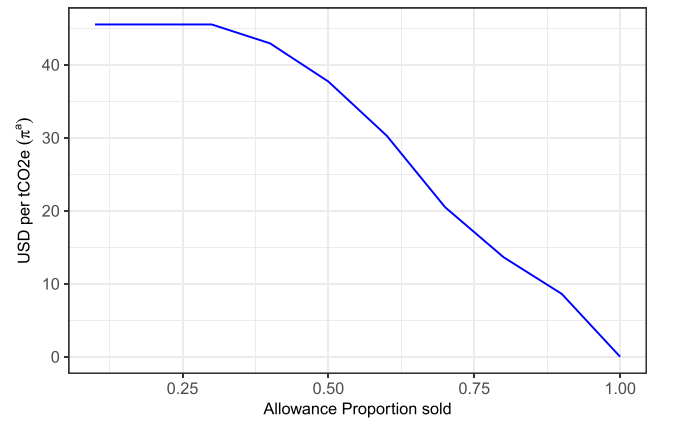
\includegraphics[width=15cm]{docs/DocumentoMemoria/images/figura 6 amigo.png}
    \caption{Venta de permisos por generador de carbón (Fuente: \protect\citeB{amigo_two_2021})}
    \label{fig:fig6}
\end{figure}


\subsubsection{Modelo sin restricciones}

Primero se evaluará el modelo al considerar únicamente la función objetivo del subastador con el costo original $\mathcal{F}$ y el costo de rendimiento. También se considera como variable de decisión únicamente los permisos $\theta$.  

\begin{equation}
\begin{array}{rrclcl}
    \displaystyle \min_{\theta} & -\theta \pi^aP + \tilde{\mathcal{F}}(P)+F(\theta)  \label{fo:perfornorest}\\
\end{array}
\end{equation}
\begin{equation}
\begin{array}{cl}
    \theta \geq 0 & (\varrho)\label{res:sub2}
\end{array}
\end{equation}

Con lo anterior se logra el siguiente Lagrangiano:

$$\mathcal{L}(\theta)=-P\theta\pi^a+\mathcal{F}(\theta)+c(P-d)^2 - \varrho\theta $$

Realizando la derivada de primer orden para $\theta$ se obtiene:

\begin{equation}
\begin{array}{rrclcl}
    \frac{\partial\mathcal{L}(\theta)}{\partial (\theta)}=-P\pi^a+\frac{\partial\mathcal{F}(\theta)}{\partial(\theta)}-\varrho=0 \label{lag1}\\
\end{array}
\end{equation}
\begin{equation}
\begin{array}{rrclcl}
    \rightarrow -P\pi^a+\frac{\partial\mathcal{F}(\theta)}{\partial(\theta)}=\varrho \label{lag1}\\
\end{array}
\end{equation}
Con esto se obtiene la siguiente complementariedad para el problema del subastador:

\begin{equation}
\begin{array}{rrclcl}
    0\leq -P\pi^a+\frac{\partial\mathcal{F}(\theta)}{\partial(\theta)}\perp \theta \geq 0 \label{compllag1}\\
\end{array}
\end{equation}

Al igual que en el modelo original de \citeB{amigo_two_2021}, se consideran los siguientes valores para constantes y parámetros:
\begin{enumerate}
    \item $\frac{\partial\mathcal{F}(\theta)}{\partial(\theta)}=0$
    \item $CAP\sim \mathcal{N}(100MtCO_{2}e,0)$
\end{enumerate}

Con esto, al correr el modelo en el \textit{solver}, cambiando únicamente el valor del rendimiento ($P$), se encontraron los siguientes resultados:

\begin{table}[H]
\centering
\begin{tabular}{|l|l|l|}
\hline
\textbf{P($\%$)} & \textbf{$\theta$ (millones)} & \textbf{$\pi^a$($\frac{\$}{\theta}$)} \\ \hline
0 & N/A & N/A \\ \hline
5 & 104 & 223 \\ \hline
10 & 3203 & 0 \\ \hline
15 & 3203 & 0 \\ \hline
20 & 3203 & 0 \\ \hline
25 & 3203 & 0 \\ \hline
30 & 3203 & 0 \\ \hline
35 & 3203 & 0 \\ \hline
40 & 3203 & 0 \\ \hline
45 & 3203 & 0 \\ \hline
50 & 3203 & 0 \\ \hline
55 & 3203 & 0 \\ \hline
60 & 3203 & 0 \\ \hline
65 & 3203 & 0 \\ \hline
70 & 3203 & 0 \\ \hline
75 & 3203 & 0 \\ \hline
80 & 3203 & 0 \\ \hline
85 & 3203 & 0 \\ \hline
90 & 3203 & 0 \\ \hline
95 & 3203 & 0 \\ \hline
100 & 1870 & 0 \\ \hline
\end{tabular}
\caption{Resultados con rendimiento y sin restricciones}
\label{tabla:sinrestr}
\end{table}


Los resultados encontrados en el Cuadro \ref{tabla:sinrestr}, pueden ser resultado de no considerar una restricción para $\theta$ respecto al presupuesto de carbono en el problema del subastador. En la siguiente subsección se desarrolla el problema incluyendo la restricción adicional.

\subsubsection{Modelo con restricción original}

Manteniendo la restricción original de \citeB{amigo_two_2021} mostrada en \ref{res:sub1}. Se tiene el siguiente modelo:

\begin{equation}
\begin{array}{rrclcl}
   \displaystyle \min_{\theta} & -\theta \pi^aP + c(P-d)^2+F(\theta) \\\textrm{s.a.} \label{eq:perforconrestr}\\
\end{array}
\end{equation}
\begin{equation}
\begin{array}{cl}
    \varphi^-1 (\varepsilon )\sigma + \mu - \theta \geq 0 & (\eta)  \label{perforconrestr:r1}
\end{array}
\end{equation}
\begin{equation}
\begin{array}{cl}
    \theta \geq 0 & (\varrho)
\end{array}
\end{equation}

Al igual que el caso anterior, se debe convertir este modelo en un MCP. Para esto se aplican las condiciones de KKT.

$$\mathcal{L}(\theta)=-P\theta\pi^a+\mathcal{F}(\theta)+c(P-d)^2 -\eta(\varphi^-1 (\varepsilon )\sigma + \mu - \theta)- \varrho\theta $$

Realizando la derivada de primer orden para $\theta$ se obtiene:

\begin{equation}
\begin{array}{rrclcl}
    \frac{\partial\mathcal{L}(\theta)}{\partial (\theta)}=-P\pi^a+\frac{\partial\mathcal{F}(\theta)}{\partial(\theta)}-\eta -\varrho=0 \label{lag20}\\
\end{array}
\end{equation}
\begin{equation}
\begin{array}{rrclcl}
    \rightarrow -P\pi^a+\frac{\partial\mathcal{F}(\theta)}{\partial(\theta)}-\eta=\varrho \label{lag21}\\
\end{array}
\end{equation}

Obteniendo la primera complementariedad:

\begin{equation}
\begin{array}{rrclcl}
    0\leq -P\pi^a+\frac{\partial\mathcal{F}(\theta)}{\partial(\theta)}-\eta \perp \theta \geq 0 \label{compllag2}\\
\end{array}
\end{equation}

La segunda complementariedad se obtiene al considera la restricción \ref{perforconrestr:r1} con su variable dual respectiva $\eta$. Obteniendo:

\begin{equation}
\begin{array}{rrclcl}
    0 \leq \varphi^-1 (\varepsilon )\sigma + \mu - \theta \perp \eta \geq 0 \label{compllag2}\\
\end{array}
\end{equation}

Nuevamente, al igual que en el modelo original de \citeB{amigo_two_2021}, se consideran los siguientes valores para constantes y parámetros:
\begin{enumerate}
    \item $\frac{\partial\mathcal{F}(\theta)}{\partial(\theta)}=0$
    \item $CAP\sim \mathcal{N}(100MtCO_{2}e,0)$
\end{enumerate}

Con esto, al correr el modelo en el \textit{solver}, cambiando únicamente el valor del rendimiento ($P$), se encontraron los siguientes resultados:

\begin{table}[H]
\centering
\begin{tabular}{|l|l|l|}
\hline
\textbf{P($\%$)} & \textbf{$\theta$ (millones)} & \textbf{$\pi^a$($\frac{\$}{\theta}$)} \\ \hline
0 & 0.3336 & 30130 \\ \hline
5 & 100 & 315.825 \\ \hline
10 & 100 & 315.825 \\ \hline
15 & 100 & 315.825 \\ \hline
20 & 100 & 315.825 \\ \hline
25 & 100 & 315.825 \\ \hline
30 & 100 & 315.825 \\ \hline
35 & 100 & 315.825 \\ \hline
40 & 100 & 315.825 \\ \hline
45 & 100 & 315.825 \\ \hline
50 & 100 & 315.825 \\ \hline
55 & 100 & 315.825 \\ \hline
60 & 100 & 315.825 \\ \hline
65 & 100 & 315.825 \\ \hline
70 & 100 & 315.825 \\ \hline
75 & 100 & 315.825 \\ \hline
80 & 100 & 315.825 \\ \hline
85 & 100 & 315.825 \\ \hline
90 & 100 & 315.825 \\ \hline
95 & 100 & 315.825 \\ \hline
100 & 100 & 315.825 \\ \hline
\end{tabular}
\caption{Resultados con rendimiento y restricción original}
\label{tabla:conrestr}
\end{table}

Del Cuadro \ref{tabla:conrestr} se entiende que al incluir únicamente las restricciones del problema original solo existe un efecto en el precio y cantidad de permisos cuando el rendimiento es 0. Pero esto no debería ocurrir ya que por lo menos se tiene la información pública $d$. Cabe notar que una cantidad de $100 MtCO_2 e$ con un precio de 315.825 USD cada una, son los valores de resolución del problema original con los mismos parámetros. Este resultado puede resultar debido a que no se a incluido una restricción que describa de mejor forma el costo de rendir.
    % archivo de apendice

%\input{apendice_b}    % otro archivo de apendice

\label{end}
\end{document}

%%%%%%%%%%%%%%%%%%%%%%%%%%%%%%%%%%%%%%%%%%%%%%%%%%%%%%%%%%%%
